% !TEX encoding = UTF-8 Unicode
\documentclass[14pt, aspectratio=169]{beamer}
\usepackage[utf8]{inputenc}
\usepackage[T1]{fontenc}

% https://www.overleaf.com/learn/latex/Beamer#Reference_guide
% Link za beamer teme

%\usetheme{Warsaw}
\usetheme{Copenhagen}
%\usecolortheme{beaver}

% opcija da se ne vide simbolcici u donjem desnom uglu
\setbeamertemplate{navigation symbols}{}

% opcija za poluvidljiv tekst kada je slajd deljen u delove
\setbeamercovered{transparent}

\title{Etički problemi u veštačkoj inteligenciji}
\author{Vukan Antić, Katarina Dimitrijević, \\ Mirjana Jočović, Aleksandar Šarbajić}
\date{Decembar 2022}

\begin{document}


\maketitle

\section{Uvod}

\begin{frame}{Uvod}
    \begin{itemize}
        \item Veštačka inteligencija je zastupljena u različitim oblastima
    \end{itemize}
    \begin{itemize}
        \item Pored brojnih prednosti, njena primena sa sobom donosi i brojne \textbf{etičke probleme}
    \end{itemize}
    \begin{itemize}
        \item Obrađeni su etički problemi u sledećim oblastima:
        \begin{itemize}
            \item Društvene mreže i zavisnost
        \end{itemize}
        \begin{itemize}
            \item Autonomna vožnja
        \end{itemize}
        \begin{itemize}
            \item Vojska
        \end{itemize}
    \end{itemize}
    
\end{frame}

% Vukan
\section{Veštačka inteligencija i društvene mreže}

\begin{frame}{Veštačka inteligencija i društvene mreže}
    \begin{itemize}
        \item Jedna od većih primena veštačke inteligencije koju svakodnevno vidjamo je u \textbf{društvenim mrežama}
    \end{itemize}
    \begin{itemize}
        \item Cilj uvek isti - korisnik što više vremena provede na toj mreži
    \end{itemize}
    \begin{itemize}
        \item Većina koristi \textbf{sisteme preporuke}
    \end{itemize}
\end{frame}

\begin{frame}{Sistemi preporuke}
    \begin{itemize}
        \item Mreža sakuplja podatke o korisniku (preference i zanimanja), i onda prikazuje sadržaj koji bi mu se verovatno dopao
    \end{itemize}
    \begin{itemize}
        \item YouTube i Spotify
    \end{itemize}
\end{frame}

\begin{frame}{YouTube}
    \begin{itemize}
        \item Mreža za redistribuciju video sadržaja koja ima svoj sistem preporuke za dalje gledanje
    \end{itemize}
    \begin{itemize}
        \item \textbf{YouTube Kids} specijalna sekcija platfore, skoncentrisana na sadržaju za decu mladjih od 12 godina
        \item Baby Shark (11.64 milijarde pregleda), Finger Family Song (najgledaniji 1.2 milijarde pregleda), i Peppa Pig
        \item Wrong Heads Disney Wrong
        Ears Wrong Legs Kids Learn Colors Finger Family 2017 Nursery Rhymes
    \end{itemize}
\end{frame}

\begin{frame}{Spotify}
    \begin{itemize}
        \item Platforma za slusašnje muzike
        \item Da bi se razlikovala od konkurencije, dodali su sistem preporuke
        \item 62\% korisnika za novu muziku saznaje preko sistema preporuke
        \item Spotify može da preporučuje koju god muziku hoće (Music Business Inside)
    \end{itemize}
\end{frame}


\begin{frame}{Zavisnost}
    \begin{itemize}
        \item U prethodnoj deceniji, sve više ljudi boluje od zavisnosti od društvenih mreža
        \item Slična bilo kojoj drugoj zavisnosti (otežan prestanak, promena raspoloženja, promena ponašanja, ...)
        \item Svaka forma validacija na društvenim mrežama (like na Facebook-u) dovodi do lučenje dopamina
        \item Iskrivljena slika o realnosti
        \item 27\% dece koja koriste društvene mreže duže od 3 sata dnevno imaju ozbiljne probleme sa mentalnim zdravljem
    \end{itemize}
\end{frame}




% Katarina
\section{Autonomna vozila}

\begin{frame}{Autonomna vozila}
    \begin{itemize}
        \item Jedna od delatnosti u kojoj se primenjuje veštačka inteligencija je \textbf{automobilska industrija}
    \end{itemize}
    \begin{itemize}
        \item Postepenim razvojem matematičkog aparata i automobilske industrije pojavila se mogućnost razvoja vozila koja imaju potpunu autonomiju
    \end{itemize}
    \begin{itemize}
        \item Postoji nekoliko stepena autonomije koje vozila mogu da imaju
    \end{itemize}
\end{frame}

\begin{frame}{Pojava etičkih problema}
    \begin{itemize}
        \item Postoje situacije u kojima \textbf{nije} moguće izbeći nesreću
    \end{itemize}
    \begin{itemize}
        \item Kako pronaći odgovarajući etički okvir na osnovu koga bi se implementirano ponašanje vozila smatralo \textbf{moralnim ponašenjem? }
    \end{itemize}
    \begin{itemize}
        \item Postoji više različitih etičkih okvira koji se mogu često sresti u literaturi: deontološka etika, utilitarizam, etika rizika...
    \end{itemize}
\end{frame}

\begin{frame}{Problem tramvaja (eng.~{\em trolley problem})}
   \begin{figure}[h!]
        \begin{center}
            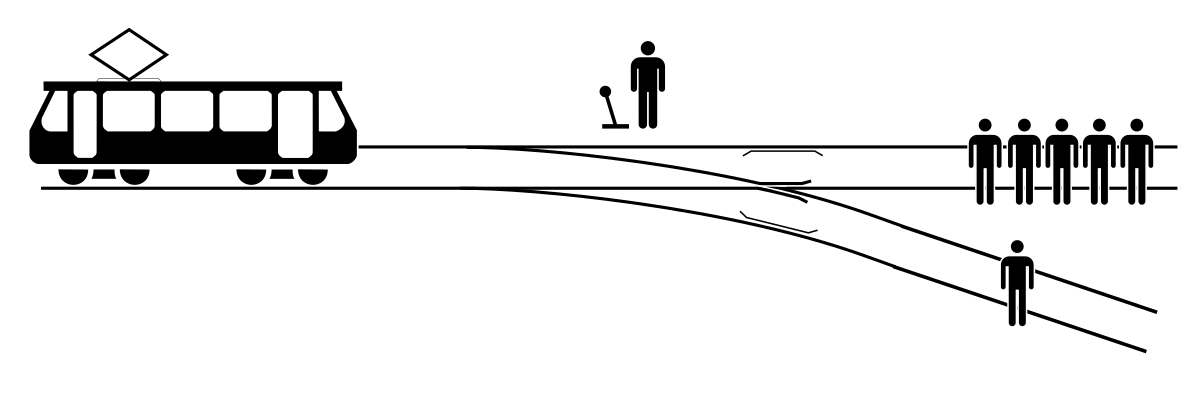
\includegraphics[scale=0.25]{Trolley_Problem.svg}
        \end{center}
        \label{fig:minAI}
    \end{figure}
\end{frame}

% Aleksandar

\section{Veštačka inteligencija u vojne svrhe}

\begin{frame}{Veštačka inteligencija u vojne svrhe}
    \begin{itemize}
    
        \item Veštačka inteligencija u vojne svrhe povlači etička pitanja
        \item \textbf{Međunarodno humanitarno pravo (IHL)} kao dodatna prepreka u razvoju etičkog softvera
        \item Veštačka inteligencija u vojne svrhe ima svoje negativne i pozitivne strane
        
    \end{itemize}
\end{frame}

\begin{frame}{Negativne strane}
    \begin{itemize}
        \item Problem odgovornosti: ko je odgovoran za dela veštačke inteligencije?
        \item Rešenje: odgovorna osoba koja odlučuje u krucijalnim trenucima
        \item Problem preprilagođenosti: nepredvidivo ponašanje algoritama usled loših trening podataka
        \item Rešenje: adekvatan odabir ulaznih podataka i algoritama za učenje, temeljno testiranje
    \end{itemize}
\end{frame}

\begin{frame}{Pozitivne strane}
    \begin{itemize}
        \item Lakše i brže osvajanje pomoću veštačke inteligencije \textbf{nije} pozitivna strana
        \item Etičko oružije u vidu \textbf{MaxAI} i \textbf{MinAI} jeste pozitivna strana
        \item MaxAI: ne izvodljiv u praksi, trudi se da što preciznije prati naređenja
        \item MinAI: naređenja koja krše zakone se jednostavno ne izvršavaju, moguće je zadavanje sekundarnog naređenja (failsafe)
    \end{itemize}    
\end{frame}

\begin{frame}{Primer etičkog oružija: MinAI}
    \begin{figure}[h!]
        \begin{center}
            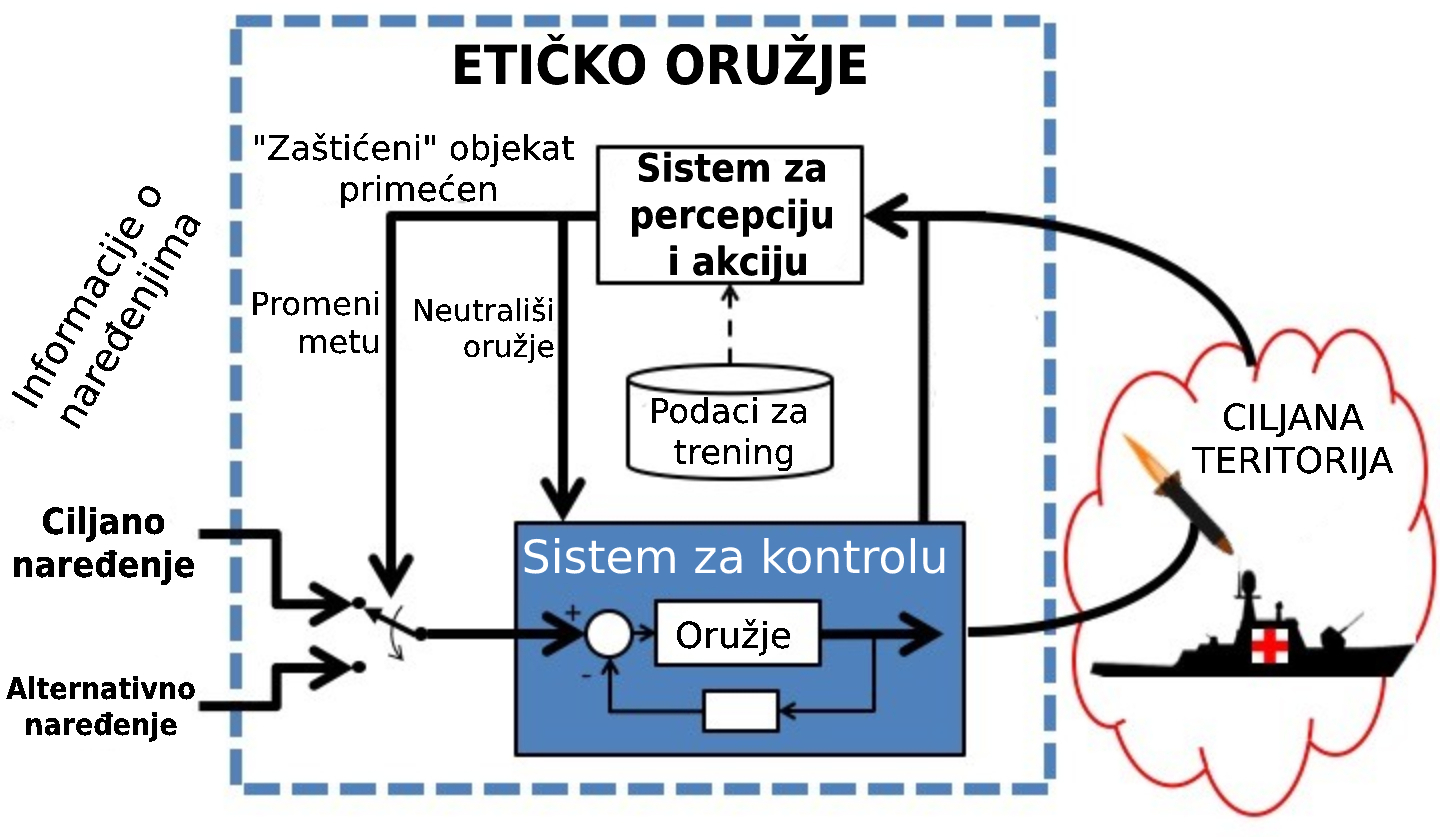
\includegraphics[scale=0.205]{minAI_slideovi.jpg}
        \end{center}
        \label{fig:minAI}
    \end{figure}
\end{frame}

\section{Zaključak}

\begin{frame}{Zaključak}
    \begin{itemize}
        \item Veštačka inteligencija i etika su kompleksne oblasti za koje je teško dati jasne odgovore
        \item Etički problemi su prisutni u mnogim oblastima pored pomenutih
        \item Detaljnija diskusija je potrebna za proučavanje etičkih problema u oblastima kao što su umetnost, radna snaga, obrada slike i zvuka, ekonomija i druge
    \end{itemize}
\end{frame}


\end{document}
